\chapter{Results}\label{chapter_4}

The following Figure~\ref{fig:spider_resnet50} shows the best macro-averaged f1-score per pre-training domain achieved with a Resnet50 model. 
The semi-transparent area indicates the sample standard deviation.

\begin{figure}[H]
    \begin{center}
    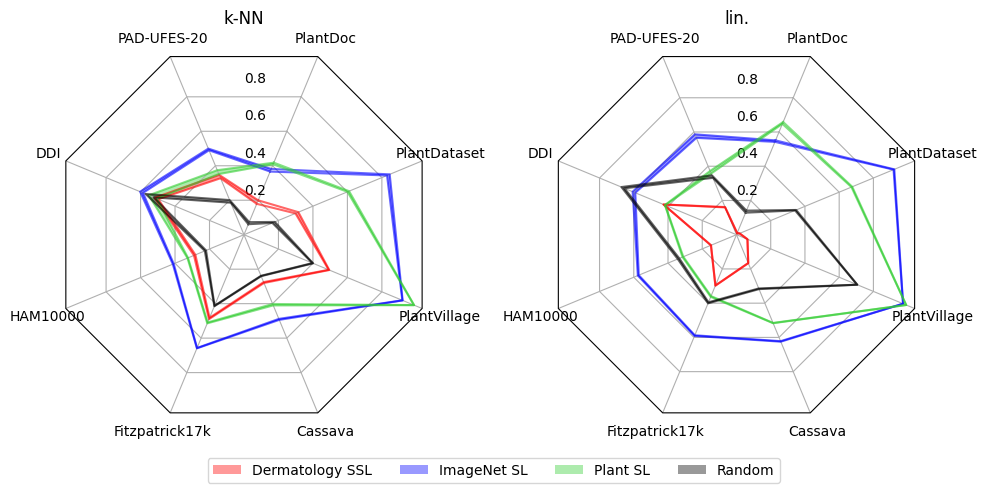
\includegraphics[width=15cm]{spider_resnet50.png}
    \caption{Frozen evaluation scores of Resnet50}\label{fig:spider_resnet50}
    \end{center}
\end{figure}

Overall the ImageNet based approach outperforms the other approaches in most cases.
PlantDoc and the \gls{pvd} are only tasks in which the plant based model actually get the best result.
The dermatology based model performs very poorly and gets beaten by the randomly initialized model in some multiple cases.
The scores are never significantly better than the other pre-trained models. 
% The model which was trained on ImageNet with \gls{ssl} was not put into the graphic, but the tables show that these scores are bad as well. 
This indicates a problem with the type of training rather than with the data per se.

The respective results of \gls{vit} models can bee seen in Figure~\ref{fig:spider_vit_t16}.

\begin{figure}[H]
    \begin{center}
    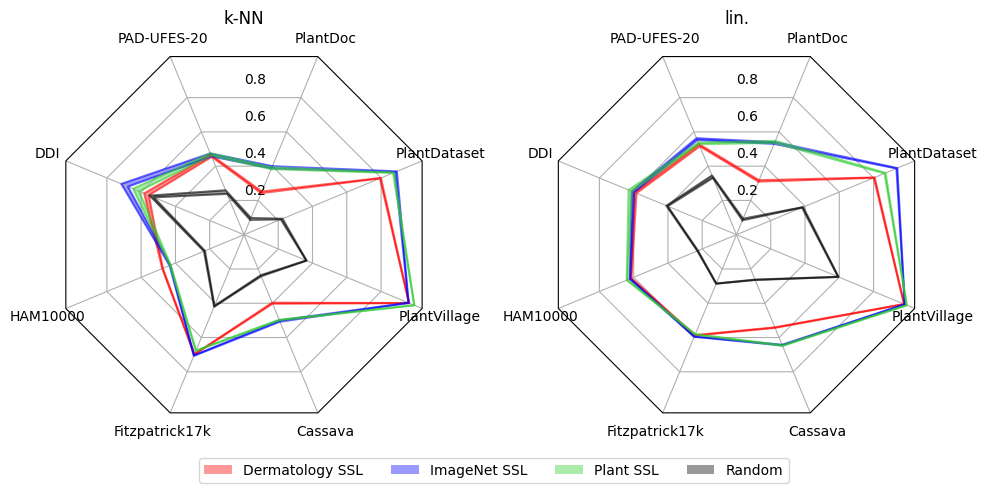
\includegraphics[width=15cm]{spider_vit_t16.png}
    \caption{Frozen evaluation of \gls{vit}}\label{fig:spider_vit_t16}
    \end{center}
\end{figure}

The scores look similar. 
The scores of the plant based model are better in some tasks than the model trained with \gls{sl} on ImageNet, but not better than the \gls{ssl} variant. 
All DINO based models are relatively close to each other. 
This is probably due to their way of training rather than the data.

% In the linear evaluation the plant based model is actually a bit better than the ImageNet based model, but with \gls{knn} the difference becomes negligible.
\section{Results on plant disease tasks}

\begin{table}[H]
    \centering
    \caption{F1-scores [\%] of Resnet50 on the plant downstream tasks\label{tab:f1_scores_resnet_plant}}
    {\fontsize{8pt}{10pt}\selectfont 
    \csvreader[tabular=|l|c|c|c|c|c|c|c|c|,
    filter expr={test{\ifnumgreater{\thecsvinputline}{3}}},
    table head=\hline\multicolumn{1}{|c|}{} & \multicolumn{2}{c|}{\bfseries PlantDoc} & \multicolumn{2}{c|}{\bfseries PlantDataset} & \multicolumn{2}{c|}{\bfseries Cassava} & \multicolumn{2}{c|}{\bfseries PlantVillage}\\\hline Pre-training & Lin. & k-NN & Lin. & k-NN & Lin. & k-NN & Lin. & k-NN \\\hline,
    table foot=\hline\multicolumn{1}{|c|}{ZeroR baseline} & \multicolumn{2}{c|}{0.3} & \multicolumn{2}{c|}{1.8} & \multicolumn{2}{c|}{15.2} & \multicolumn{2}{c|}{0.5}\\\hline]{../../results/f1_scores_resnet_plant.csv}{}%
    {\csvcoli\ & \csvcolii & \csvcoliii & \csvcoliv & \csvcolv & \csvcolvi & \csvcolvii & \csvcolviii & \csvcolix}%
    }
\end{table}
\begin{table}[H]
    \centering
    \caption{F1-scores [\%] of ViT-T16 on the plant downstream tasks\label{tab:f1_scores_vit_plant}}
    {\fontsize{8pt}{10pt}\selectfont 
    \csvreader[tabular=|l|c|c|c|c|c|c|c|c|,
    filter expr={test{\ifnumgreater{\thecsvinputline}{3}}},
    table head=\hline\multicolumn{1}{|c|}{} & \multicolumn{2}{c|}{\bfseries PlantDoc} & \multicolumn{2}{c|}{\bfseries PlantDataset} & \multicolumn{2}{c|}{\bfseries Cassava} & \multicolumn{2}{c|}{\bfseries PlantVillage}\\\hline Pre-training & Lin. & k-NN & Lin. & k-NN & Lin. & k-NN & Lin. & k-NN \\\hline,
    table foot=\hline\multicolumn{1}{|c|}{ZeroR baseline} & \multicolumn{2}{c|}{0.3} & \multicolumn{2}{c|}{1.8} & \multicolumn{2}{c|}{15.2} & \multicolumn{2}{c|}{0.5}\\\hline]{../../results/f1_scores_vit_plant.csv}{}%
    {\csvcoli\ & \csvcolii & \csvcoliii & \csvcoliv & \csvcolv & \csvcolvi & \csvcolvii & \csvcolviii & \csvcolix}%
    }
\end{table}

All f1-scores on the plant disease tasks are listed in Table~\ref{tab:f1_scores_resnet_plant} for Resnet50 and Table~\ref{tab:f1_scores_vit_plant} for \gls{vit} respectively.
The numbers show the mean macro-averaged f1-scores as percentage with the sample standard deviation.
The ZeroR baseline represents a dummy classifier always predicting the largest class regardless of the input data.
The deviation for the baseline was omitted, because this classifier is unaffected by randomness.


\subsection{PlantDoc}
The best results for the PlantDoc task is pre-trained on plant images. 
This is true for Resnet50 as well as the \gls{vit} models.
SimCLR was used to pre-train the Resnet50 models on ImageNet and dermatology images and both of these models perform poorly.
\gls{sl} with ImageNet achieves significant better scores, making thus clear, that the training algorithm can have a high impact on the results. 

Figure \ref{fig:lines_plantdoc} shows the macro-averaged f1-scores when the training data gets reduced.
The subsampling was repeated 100 times with different random seeds. 
Thus, the standard deviation is higher compared to the full dataset.

\begin{figure}[H]
    \begin{center}
    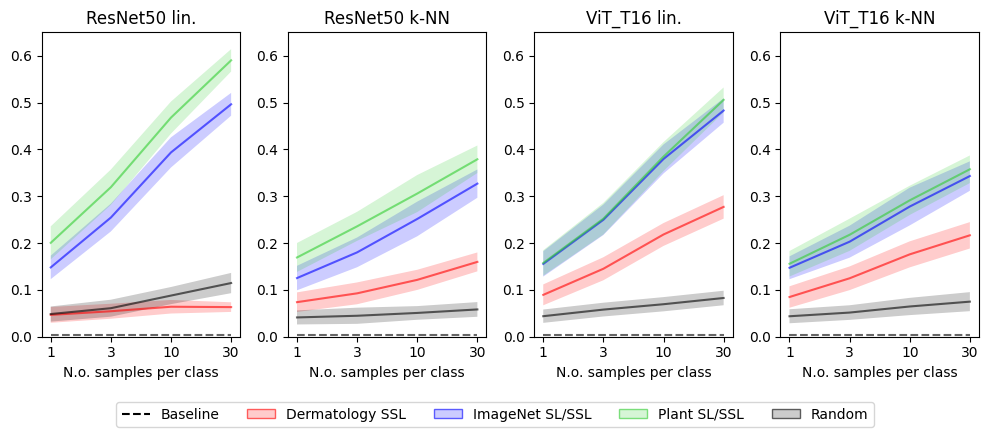
\includegraphics[width=15cm]{lines_plantdoc.png}
    \caption{F1-scores of frozen evaluation on subsampled sets on PlantDoc}\label{fig:lines_plantdoc}
    \end{center}
\end{figure}

\subsection{PlantDataset}
Figure \ref{fig:lines_plantdataset} presents the same evaluation for the PlantDataset task.
\newacronym{knn}{k-NN}{k-nearest neighbors}
The ImageNet based model clearly dominate using the linear classifier as well as \gls{knn}.
% SimCLR performs similarly bad
\begin{figure}[H]
    \begin{center}
    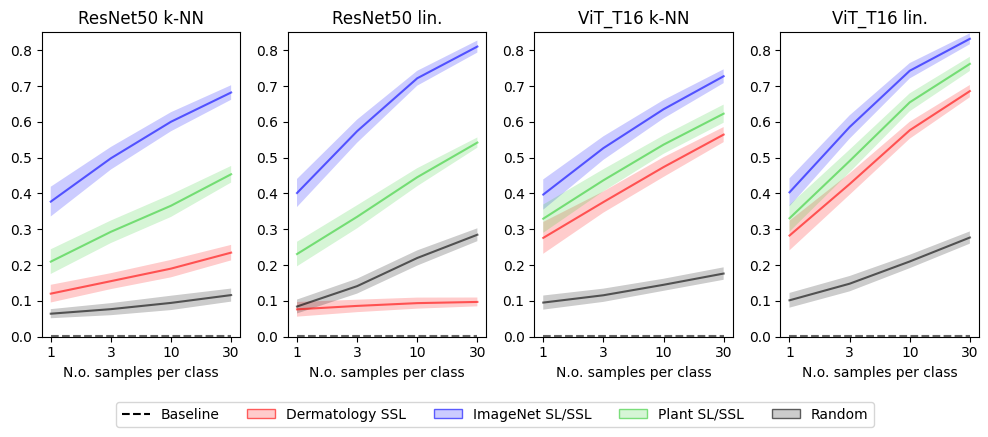
\includegraphics[width=15cm]{lines_plantdataset.png}
    \caption{F1-scores of frozen evaluation on subsampled sets on PlantDataset}\label{fig:lines_plantdataset}
    \end{center}
\end{figure}

\subsection{Cassava Leaf Disease Classification}
The Cassava dataset is large enough to subsample up tp a 100 images per class as shown in Figure \ref{fig:lines_cassava}.
\gls{knn} produces a clearly worse result with the model based on \gls{pddd} than the linear evaluation does.
The selected values for $k$ are on average very high, which suggests overfitting as cause.
ImageNet and plant images are about equally suitable with the \gls{vit}.

\begin{figure}[H]
    \begin{center}
    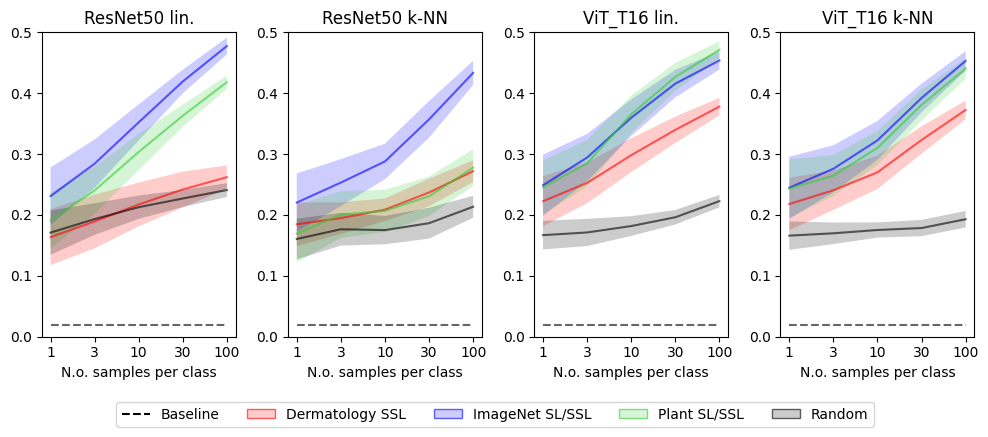
\includegraphics[width=15cm]{lines_cassava.png}
    \caption{F1-scores of frozen evaluation on subsampled sets on Cassava}\label{fig:lines_cassava}
    \end{center}
\end{figure}

\subsection{PlantVillage Dataset (PVD)}
The f1-scores on the \gls{pvd} are by far the highest ones of all downstream tasks. 
The plant based models clearly surpass the other models and emphasize the impact of transfer learning.
Figure \ref{fig:lines_plantvillage} also shows the clear separation between the different models.
Both effects could be made possible by the amount of data, since this dataset is the largest and has the highest number of classes. 

\begin{figure}[H]
    \begin{center}
    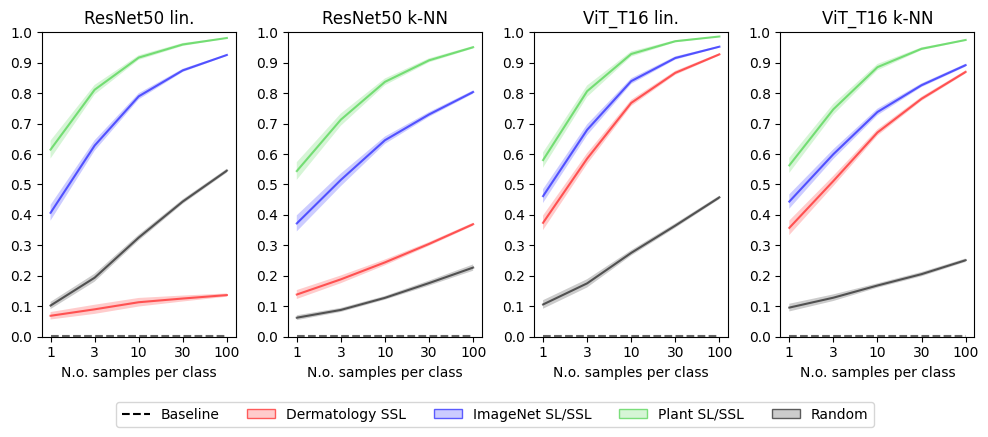
\includegraphics[width=15cm]{lines_plantvillage.png}
    \caption{F1-scores of frozen evaluation on subsampled sets on \gls{pvd}}\label{fig:lines_plantvillage}
    \end{center}
\end{figure}

\section{Results on skin disease tasks}
Table~\ref{tab:f1_scores_resnet_derma} and Table~\ref{tab:f1_scores_vit_derma} lists the f1-scores for the dermatology tasks. 
While plant based models come off very well in their downstream tasks, this is not the case with the skin disease models. 
The \gls{knn} evaluation of the \gls{vit} on the HAM10000 dataset is the only case where the dermatology model narrowly beats the other.

%Write here about the clustering of DINO

\begin{table}[H]
    \centering
    \caption{F1-scores [\%] of Resnet50 on dermatology downstream tasks\label{tab:f1_scores_resnet_derma}}
    {\fontsize{8pt}{10pt}\selectfont 
    \csvreader[tabular=|l|c|c|c|c|c|c|c|c|,
    filter expr={test{\ifnumgreater{\thecsvinputline}{3}}},
    table head=\hline\multicolumn{1}{|c|}{} & \multicolumn{2}{c|}{\bfseries DDI} & \multicolumn{2}{c|}{\bfseries PAD-UFES-20} & \multicolumn{2}{c|}{\bfseries HAM10000} & \multicolumn{2}{c|}{\bfseries Fitzpatrick17k}\\\hline Pre-training & Lin. & k-NN & Lin. & k-NN & Lin. & k-NN & Lin. & k-NN \\\hline,
    table foot=\hline\multicolumn{1}{|c|}{ZeroR baseline} & \multicolumn{2}{c|}{42.6} & \multicolumn{2}{c|}{8.9} & \multicolumn{2}{c|}{10.7} & \multicolumn{2}{c|}{28.1}\\\hline]{../../results/f1_scores_resnet_derma.csv}{}%
    {\csvcoli\ & \csvcolii & \csvcoliii & \csvcoliv & \csvcolv & \csvcolvi & \csvcolvii & \csvcolviii & \csvcolix}%
    }
\end{table}

\begin{table}[H]
    \centering
    \caption{F1-scores [\%] of ViT-T16 on dermatology downstream tasks\label{tab:f1_scores_vit_derma}}
    {\fontsize{8pt}{10pt}\selectfont 
    \csvreader[tabular=|l|c|c|c|c|c|c|c|c|,
    filter expr={test{\ifnumgreater{\thecsvinputline}{3}}},
    table head=\hline\multicolumn{1}{|c|}{} & \multicolumn{2}{c|}{\bfseries DDI} & \multicolumn{2}{c|}{\bfseries PAD-UFES-20} & \multicolumn{2}{c|}{\bfseries HAM10000} & \multicolumn{2}{c|}{\bfseries Fitzpatrick17k}\\\hline Pre-training & Lin. & k-NN & Lin. & k-NN & Lin. & k-NN & Lin. & k-NN \\\hline,
    table foot=\hline\multicolumn{1}{|c|}{ZeroR baseline} & \multicolumn{2}{c|}{42.6} & \multicolumn{2}{c|}{8.9} & \multicolumn{2}{c|}{10.7} & \multicolumn{2}{c|}{28.1}\\\hline]{../../results/f1_scores_vit_derma.csv}{}%
    {\csvcoli\ & \csvcolii & \csvcoliii & \csvcoliv & \csvcolv & \csvcolvi & \csvcolvii & \csvcolviii & \csvcolix}%
    }
\end{table}


\subsection{Diverse Dermatology Images (DDI)}
The \gls{ddi} dataset was used for a binary classification. 
Additionally, one class has significantly more images than the other.
This bias causes an unusually high baseline score, as can be seen in Figure~\ref{fig:lines_ddi}.

\begin{figure}[H]
    \begin{center}
    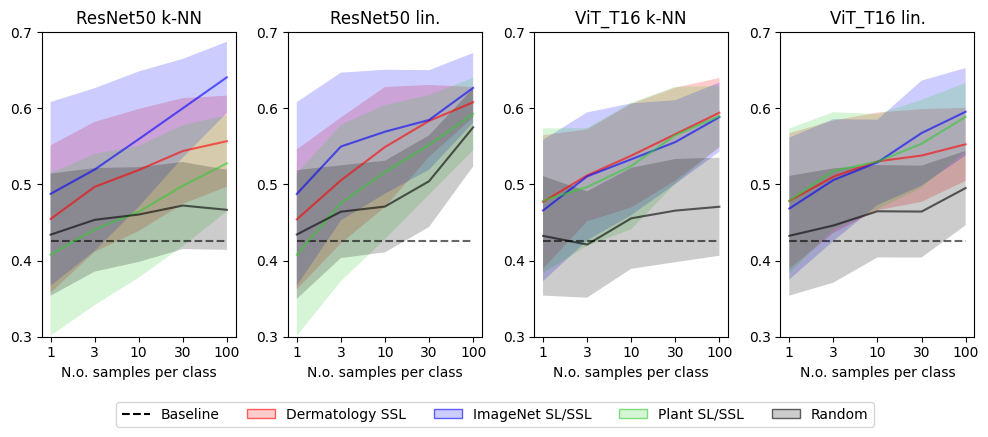
\includegraphics[width=15cm]{lines_ddi.png}
    \caption{F1-scores of frozen evaluation on subsampled sets on \gls{ddi}}\label{fig:lines_ddi}
    \end{center}
\end{figure}

\subsection{PAD-UFES-20}
Figure~\ref{fig:lines_pad-ufes-20} shows a difference between the two architectures. 
While the results with Resnet50 are spread out, the models trained with DINO all behave very alike.
\begin{figure}[H]
    \begin{center}
    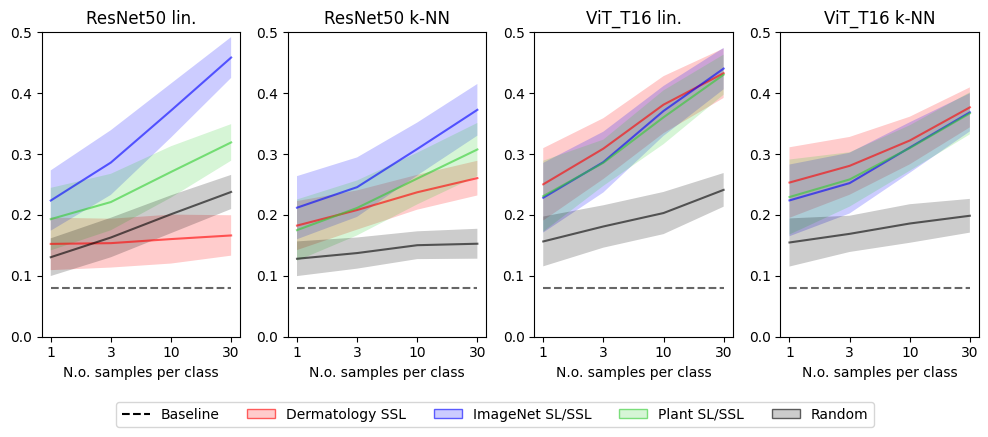
\includegraphics[width=15cm]{lines_pad-ufes-20.png}
    \caption{F1-scores of frozen evaluation on subsampled sets on PAD-UFES-20}\label{fig:lines_pad-ufes-20}
    \end{center}
\end{figure}

\subsection{HAM10000}
A similar situation occurs with the f1-scores on the HAM10000 dataset in Figure~\ref{fig:lines_ham10000}.
The graphs of the models trained with DINO are somewhat close together and still overlap with 100 images per class.
Although some \gls{isic} images were included in the pre-training it did not lead to an obvious advantage.
%TODO promising?
\begin{figure}[H]
    \begin{center}
    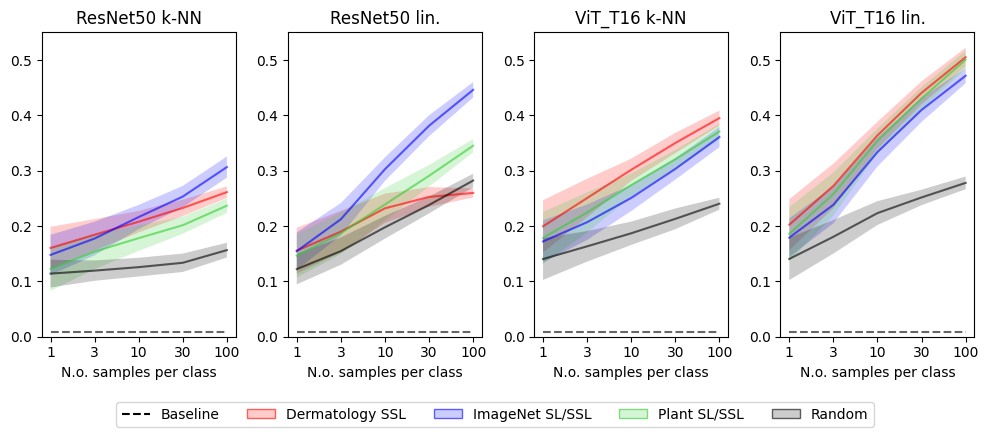
\includegraphics[width=15cm]{lines_ham10000.png}
    \caption{F1-scores of frozen evaluation on subsampled sets on HAM10000}\label{fig:lines_ham10000}
    \end{center}
\end{figure}

\subsection{Fitzpatrick17k}
The results on the Fitzpatrick17k dataset shown in Figure~\ref{fig:lines_fitzpatrick17k} do not look promising.
The DINO models are overlapping each other indistinguishable.
\begin{figure}[H]
    \begin{center}
    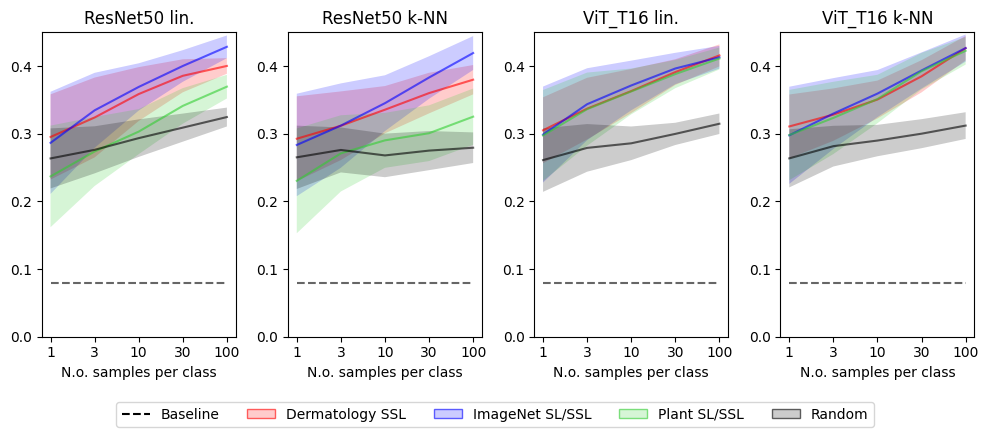
\includegraphics[width=15cm]{lines_fitzpatrick17k.png}
    \caption{F1-scores of frozen evaluation on subsampled sets on Fitzpatrick17k}\label{fig:lines_fitzpatrick17k}
    \end{center}
\end{figure}


% \section{Other}
% \subsection{DINO student/teacher}
% \subsection{Fine-tuning}
% \subsection{Fine-tuning}
